\documentclass[11pt]{article}
\include{noteinclude}
\include{natbib}

\begin{document}
\tableofcontents

\section{Introduction}

This document provides a guide to using Matthew Burger's neutral cloud model.
You can contact me at 
\href{mailto:Matthew.Burger@nasa.gov}{Matthew.Burger@nasa.gov}. 

The document is organized as follows:
\begin{enumerate}
\item Setting things up: how to get the model running on your computer
\item Creating Packets
  \begin{enumerate}
  \item Creating Input files
  \item Running the model
  \end{enumerate}
\item Displaying outputs
  \begin{enumerate}
  \item Creating format files
  \item produce\_results
  \end{enumerate}
\item What the model does: I try to explain the physical and computational 
processes in more detail and provide examples to prove it works the way it 
should.
\item Program Catalog: Help file and algorithm description for each program.
\end{enumerate}

\section{Setup}

All of the files used for the model are listed in Appendix A. Everything
necessary for running the model is synced to the LASP server
\texttt{mascs\_data} in the directory \texttt{Burger/NeutralModel/}. This
contains the following directories:
\begin{enumerate}
\item \texttt{modelpro} \rarrow\ all the model code
\item \texttt{misc} \rarrow\ various helper functions including the IDL
Astronomy Library and the ICY SPICE Library (SPICE for IDL)
\item \texttt{spice\_kernels} \rarrow\ The SPICE kernels necessary for
comparing model runs with MESSENGER data
\item \texttt{SummaryFiles} \rarrow\ The UVVS summary files created by Aimee
Merkel.
\end{enumerate}

Start IDL and compile the model by typing: 
\begin{verbatim}
    IDL> @PATH/compile_model_mercury
\end{verbatim}

The routines \textit{physical\_constants} and textit{PlanetaryConstants} will 
set up a series of system variables with various physical constants and 
planetary data. The new
system variables are: \texttt{!consts}, \texttt{!Sun}, \texttt{!Mercury}, ...
\texttt{!Pluto}. To see what is contained in each variable, type: \\
\hspace*{1cm}\texttt{IDL> help, /struct,} \textit{variable}

\section{Input Files}

The input file contains all the parameters needed to run the model. This should 
be all you need to change to get the output you are looking for. The file 
contains a series of lines in the format: \\
\hspace*{1cm} \textit{structure.field} = \textit{value}  \\
String values should not have quote marks around them. Numerical values cannot 
be mathematical operations. For numerical values, it is not necessary to 
specify double precision. All the inputs are case insensitive. I use 
capitalization to make things clearer for me, but it is not necessary.

The inputs and outputs are contained in a series of structures. The input 
structures are:
\begin{enumerate}
\item geometry
\item sticking\_info
\item forces
\item SpatialDist
\item SpeedDist
\item AngularDist
\item PerturbVel
\item plasma\_info
\item options
\end{enumerate}
This may seen like a lot of structures, but I've found that this allows a large 
number of options to be set while still keeping things organized. In the 
sections that follow, I descirbe each structure and give the possible options. 
Fields in red are optional. If a required field is not included in the input 
file, the run will crash. Appendix B summarizes the options.

\subsection{geometry}

The format of the geometry structure depends on the central object in the 
system. 

\begin{enumerate}
\item Mercury
  \begin{enumerate}
  \item planet = Mercury
  \item taa = true anomaly angle in radians
  \item {\color{red}include} = 1/0 depending on whether to include Mercury's 
  gravity as a force. (Default = 1)
  \end{enumerate}
\item Earth
  \begin{enumerate}
  \item planet = Earth
  \item StartPoint = Earth or Moon
  \item phi = final heliocentric orbital position for the Earth and Moon. The Earth's
  position is currently ignored, although I need to add in seasonal effects. This line
  needs to be included either 1 or 2 times. If only included once, then it is assumed to
  be for the moon.
  \item {\color{red}include} = 1/0 depending on whether to include the gravity from the
  Earth and moon. If present, must be included twice. Default = 1 for each object. 
  \end{enumerate}
\item Jupiter
  \begin{enumerate}
  \item planet = Jupiter
  \item StartPoint = Jupiter or one of its moons
  \item CML = central meridian longitude in radians
  \item phi = final heliocentric orbital position for the planet and each moon. 
  The line \texttt{geometry.phi = xxx} must be included 5 times (one time each 
  for Jupiter, Io, Europa, Ganymede, and Callisto, in order). The orbital 
  position for Jupiter is always 0, so this line doesn't matter, although it 
  must be included. 
  \item {\color{red}include} = 1/0 depending on whether to include the gravity 
  from Jupiter and each moon as a force. This line must be included 5 times. 
  Default = 1 for all objects.
  \end{enumerate}
\item Saturn
  \begin{enumerate}
  \item planet = Saturn
  \item StartPoint = Saturn or one of its moons
  \item phi = final heliocentric position for the planet and each moon. This 
  line must be included 10 times (one time each for Saturn, Mimas, Enceladus, 
  Tethys, Dione, Rhea, Titan, Hyperion, Iapetus, and Phoebe, in order).
  \item {\color{red}include} = 1/0 depending on whether to include gravity from 
  each object. This line must be included 10 times. Default = 1 for each object.
  \end{enumerate}
\end{enumerate}

Regarding the \textit{include} option: In general it is only necessary to 
include the gravity from the central object and the starting satellite. 
Including more satellites has little effect on particle trajectories over short 
time scales and will slow things down since more computations are necessary.

\subsection{sticking\_info}

This structure controls what happens when when a packet hits the surface. 
Currently the sticking coefficient is a constant, but I will add more 
complicated functions. If the sticking coefficeint equals 1, then the entire 
packet sticks to the surface and the integration is complete. If it is less 
than 1, the additional fields in \textit{sticking\_info} specify how the packet 
is reemitted from the surface.

\begin{enumerate}
\item StickCoef = a number between 0 and 1 to specify the fraction of the 
packet which sticks to the surface. 
\item If StickCoef = 1, then nothing else is required.
\item If StickCoef $<1$, then the following options are possible:
  \begin{enumerate}
  \item Thermal accommodation to the surface temperature. The packet is reemitted in a
  random direction at a speed between the incident speed and random speed based on the
  local surface temperature. The new velocity is $v_1 = a v' + (1-a)v_0$, where $v'$ is
  chosen from the Maxwellian disrtibution function $f_M(v,T)$.
    \begin{itemize}
    \item emitfn = Maxwellian
    \item Tsurf = surface temperature (K). If Tsurf=0, then the local surface
    temperature is computed as a function of solar zenith angle (only set up for
    Mercury). Otherwise, the surface temperature is assumed constant.
    \item accom\_factor = a number between 0 and 1 indicating the amount of thermal
    accommodation (1 = fully accommodated).
    \end{itemize}
  \item Elastic scattering. The packet is reemitted in a random direction at 
  the same speed it hit the surface with. This is equivalent to setting emitfn to
  Maxwellian and accom\_factor = 0 (no accommodation).
    \begin{itemize}
    \item emitfn = elastic scattering
    \end{itemize}
  \end{enumerate}
\end{enumerate}

\subsection{forces}

This structure controls which forces acting on the packets are computed. The 
possible forces are gravity, radiation pressure, and the Lorentz force. The 
Lorentz force doesn't work right now, and in any case is irrelevant for 
neutrals. Any force not explicitly listed in the input file is turned off.

Right now I have g-values for C, Ca, Ca$^+$, H, He, K, Mg, Mg$^+$, Na, OH, O, 
and S. If radiation pressure is set for any other species, then the g-value is 
assumed to be 0.

\begin{itemize}
\item {\color{red}gravity} = 1/0 to turn gravity on/off (default = 0)
\item {\color{red}radpres} = 1/0 to turn radiation pressure on/off (default = 0)
\item {\color{red}lorentz} = 1/0 to turn the Lorentz force on/off (default = 0)
\end{itemize}

\subsection{SpatialDist}

This determines the initial spatial distribution of the packets. Currently, the 
options are: surface, torus, exosphere, and SO$_2$ exosphere. The required 
fields for each of these options are different.

There is an option called \textit{random\_even} included in each of these
distributions which used to toggle between randomly choosing packets with the
specified parameters or evenly distributing them throughout the region. The
flag is still there, but only the random option works. It turns out that evenly
distributing packets over a sphere is difficult and not really very useful.

\begin{enumerate}
\item Surface distribution. This distributes packets randomly over the surface
of a sphere. There are two ways to specify how packets are distributed: by
specifying a longitude/latitude range, or by supplying a probibility
distribution function map.

To specify a longitude and latitude range, the parameters are:
  \begin{itemize}
  \item use\_map = 0
  \item {\color{red}exobase} = radius of the sphere in units of the starting 
  point (satellite or planet) radius. Default = 1, for starting at the
  surface. Exobase $<1$ will cause problems.
  \item {\color{red}longitude0} = lower bound on lonigutde [radians]. Default =
  0.
  \item {\color{red}longitude1} = upper bound on longitude [radians]. Default =
  6.2831853.
  \item {\color{red}latitude0} = lower bound on latitude [radians]. Default = 
  -1.5707963
  \item {\color{red}latitude1} = upper bound on latitude [radians]. Default = 
  1.5707963
  \end{itemize}
The latitude range is $-\pi/2$ to $\pi/2$. The longitude range is 0 to $2\pi$.
To choose a sub-region that spans the 0 longitude,  set longitude0 $>$
longitude1. (Setting a negative value will most likely not work right - I
haven't checked.)

The probability distribution functions for longitude ($\lambda$) and 
latitude ($\mu$) are determined by:
\begin{eqnarray}
f_\lambda & \propto & constant, \lambda_0 \leq \lambda \leq \lambda_1 \\
f_\mu & \propto & cos(\mu), \mu_0 \leq \mu \leq \mu_1 
\end{eqnarray}

I need to verify that this works according
to the coordinate systems defined in Section~\ref{sec:coordsystems} below,
which are centered on the subsolar point, in the case of planets, and the
sub-planet point in the case of satellites. (Because the planetary coordinate
systems are right-handed and the satellite systems are left-handed, I expect
that there are currently some mistakes).

If you would like to specify a more complicated surface distribution, you need
to provide a mapfile in a format which I will describe later.

\item PSD. This distributes packets randomly over the surface of a sphere with
a probability that depends on the incident photon flux and the proton
precipitation flux. The PSD flux at each point on the surface is given by 
\begin{eqnarray}
\Phi_{PSD}(\lambda,\mu) & = & min \left\{\Phi_{p-l}, \Phi_{d-l} \right\} \\
\Phi_{p-l}(\lambda,\mu) & = & 
  \left(\frac{\phi_{phot}(1~\mathrm{AU})}{r^2}\right) \times 
  \cos(SZA) \times \sigma_{PSD}(T(\lambda,\mu)) \times c(\lambda,\mu) 
  n(\lambda,\mu) \\ 
\Phi_{d-l}(\lambda,\mu) & = & \phi_{diff}(\lambda,\mu) \times \left( 1 + 
  10^{-8} \kappa \phi_{precip}\right)
\end{eqnarray}
where $\lambda,\mu$ are the longitude and latitude measured relative to the
subsolar point, $\Phi_{PSD}$ is the PSD flux from the surface, and 
$\Phi_{p-l}$ and $\Phi_{d-l}$ are the photon- and diffusion-limited fluxes
respectively. 

The photon-limited flux depends on the photon flux $\phi_{phot}$ at Mercury's 
heliocentric ($r$), the solar zenith angle ($SZA$), the temperature dependent
PSD cross section ($\sigma_{PSD}$), the concentration of desorbed species (c), 
and the surface density of the regolith (n). While $\sigma$, $c$, and $n$
likely all vary with over the surface due to temperature variations and local
geology, we assume constant values of $\sigma=3\times10^{-21}$ cm$^{-2}$,
$c=0.005$, and $n=7.5\times10^{14}$ as used by \cite{burger2010}. More
complicated functions will be implemented as needed. At 1 AU, the photon flux
at energies greater than 4 eV (wavelength $<$ 310 nm), the threshold for PSD is
$\sim2.8\times10^{15}$ photons cm$^{-2}$ s$^{-1}$, which we use as a baseline
solar flux (this can potentially be parameterized if necessary).
$\cos(SZA)$ is equivalent to $\cos \lambda \cos \mu$ (demonstrated on 
Section~\ref{sec:cossza} below), and is zero on the nightside where there is no 
solar flux. 

The diffusion-limited flux is the rate at which atoms naturally diffuse from
the interior of regolith grains to their exteriors. The temperature and
compositional dependencies are not known; we assume the value is constant.
Previous estimates \cite{burger2010,killen2005} have found that $\phi_{diff}
\sim\; 10^6 - 10^7$. $\kappa$ is the ion-enhanced diffusion effectiveness, a
parameter which governs how effective precipitating ions are at increasing the
diffusion of atoms to grain surfaces. The factor of $10^{-8}$ keeps $\kappa
\sim\; 1$. 

The PSD spatial distribution is normalized such that the total source rate can
be determined by a linear fit to the data:
\begin{equation}
f_{PSD} \propto min \left\{1, \rho \times \left(1 + 10^{-8} \kappa \phi_{precip}
\right) \right\}
\end{equation}
where $\rho = \Phi_{p-l,ss}/\phi_{diff}$ is the ratio of the photon limited
flux at the sub-solar point to the diffusion limited flux. The advantage of
this construction is that the modeled source rate determines both the
photon-limited and diffusion-limited flux; the disadvantage is that $\rho$ must
be specified \textit{a priori} and a separate model run is needed for each
value of $\rho$ that may be chosen. The is no simple way around this as the
total PSD flux is not a simple linear combination of the non-enhanced and
ion-enhanced PSD fluxes. 

The total source rate is given by: 
\begin{equation}
S = \int_\Omega \Phi_{PSD} d\Omega = \int_0^{2\pi} \int_{-\pi/2}^{\pi/2} 
  \Phi_{PSD} \sin \mu d\mu d\lambda
\end{equation}
The function \texttt{PSD\_flux} does something useful to convert between fluxes
and total source rates.

The required inputs for the PSD spatial distribution are:
  \begin{itemize}
  \item $\rho$ = ratio of photon-limited and non-ion enhanced diffusion flux at
  the sub solar point
  \item $\kappa$ = effectiveness of ion-enhanced diffusion
  \item modnum = Ion precipitation model calculated by Mehdi Benna.
  \end{itemize}

The parameter modnum refers to one of the MHD model simulations computed by
Mehdi Benna; the ion precipitation flux to the surface is calculated as a
function of solar wind ion density and IMF $B_x$, $B_y$, and $B_z$. For each
MESSENGER orbit, six ion precipitation scenarios are given corresponding to two
IMF configurations (measured before MESSENGER's inbound passage through the bow
shock and after the outbound passage) and low (10 \cc), medium (20 \cc), and
high (30 \cc) solar wind densities. The function 
\textit{precipitation\_modelnum} gives the model number to use as a function of
orbit and SW configuration; a complete listing is given in the file XXXXXX. \\
\verb+IDL> modnum = precipitation_modelnum(orbit, mnum)+ \\
where \textit{mnum} refers to the conditions in Table~\ref{table:mnum}.
\begin{table}
\begin{center}
\begin{tabular}{c|c}
\textbf{mnum} & \textbf{SW conditions} \\ \hline
0 & inbound IMF, $n_i=10$ \cc \\
1 & inbound IMF, $n_i=20$ \cc \\
2 & inbound IMF, $n_i=30$ \cc \\
3 & outbound IMF, $n_i=10$ \cc \\
4 & outbound IMF, $n_i=20$ \cc \\
5 & outbound IMF, $n_i=30$ \cc
\end{tabular} \end{center}
\caption{Values for \textit{mnum} in function \texttt{precipitation\_modelnum}}
\label{table:mnum}
\end{table}

\item Torus. This begins packets in a longitudinally symmetric torus in the
equatorial plane of the central planet. The locations of packets are determined
by:
\begin{eqnarray}
x & = & (r_0 + a \cos \theta) \cos \phi \\
y & = & (r_0 + a \cos \theta) \sin \phi \\
z & = & b \sin \theta
\end{eqnarray}
where $a$, $b$, $\theta$, and $\phi$ are random variables in the ranges:
\begin{eqnarray}
0 & \leq a \leq & r_1 \\
0 & \leq b \leq & r_2 \\
0 & \leq \theta \leq & 2\pi \\
0 & \leq \phi \leq & 2\pi \\
\end{eqnarray}
This produces a torus with a major axis $r_0$, and minor axes $r_1$ in the
equatorial plane and $r_2$ out of the equatorial plane. 

Right now this can only create a torus around the central planet, although we
may want to change that later to simulate production from the Rhea ring, for
example.

Parameters:
  \begin{itemize}
  \item radius0 = torus major axis, $r_0$ [planetary radii]
  \item radius1 = torus minor axis, $r_1$ [planetary radii]
  \item radius2 = torus minor axis, $r_2$ [planetary radii]
  \end{itemize}

Add some figures showing that this works.

\item Exosphere distribution. This starts packets in a spherically symmetric
exosphere centered on the starting planet or moon. The exosphere can drop off
either exponentially or as a powerlaw. The radial components of the powerlaw
and exponential exospheres have the form: 
\begin{eqnarray}
f_r & \propto & r^b; powerlaw \\
f_r & \propto & e^(-(r-1)/b; exponential 
\end{eqnarray}
For a powerlaw exosphere, b is the powerlaw index. For an exponential
exosphere, b is the scale height. The angular components are isotropically
distributed:
\begin{eqnarray}
f_\theta & \propto & \cos \theta \\
f_\phi & \propto & constant
\end{eqnarray}
To simulate production of atomic species by photodissociation of a molecular
exosphere, there is an option (block\_shadow) to only start packets in sunlight.

Parameters:
  \begin{itemize}
  \item exotype = exponential or powerlaw
  \item b = scale height [object radii] for the exponential or powerlaw index.
  The powerlaw index should be $<0$.
  \item {\color{red}rmax} = cutoff distance for exosphere [object radii]. 
  Default = 10.
  \item {\color{red}block\_shadow} = 0/1 to allow/block packets to start in the
  geometric shadow. Default = 0.
  \end{itemize}

\item SO$_2$ exosphere. This was sent to me by Vincent Dols to simulate
production of O in Io's SO$_2$ exosphere.
\begin{eqnarray}
f_\phi & \propto & e^{-(|\phi|-\pi)^2/1.07^2} \\
f_r & \propto & -474.8 + 148.7r + 200.7 r^2 \times
  \frac{0.09}{(r_{peak}(\phi)-r^2)^2} + 0.09^2 \\
r_{peak} & = & 1.42 \times \left[1 + 0.05 \left(\frac{\pi
  -|\phi|}{\pi/4}\right)^2 \right] \\
f_{\theta} & \propto & \cos \theta
\end{eqnarray}

There are no parameters to set. 

Need to add a figure showing what this looks like.

\end{enumerate}

\subsection{SpeedDist}

Options for the SpeedDist.type are: Gaussian, trigaussian, sputtering,
Maxwellian (thermal), flat (constant), circular orbits, dolsfunction, and
user defined.

\begin{enumerate}
\item Gauusian distribution. The Gaussian speed distribution has the form:
\begin{equation}
f_v(v) \propto e^{-(v-v_{prob})^2/2/\sigma^2}
\end{equation}

Parameters are:
  \begin{itemize}
  \item vprob = most probable velocity [km/s]
  \item sigma = Gaussian width [km/s]
  \end{itemize}

\item Tri-gaussian distribution. This allows you to set a different Gaussian
speed distribution in the x, y, and z directions. This needs to be tested. I am
not sure what coordinate system is used.

Parameters are:
  \begin{itemize}
  \item vxprob = most probable speed along x axis [km/s]
  \item vxsigma = Gaussian width in x direction [km/s]
  \item vyprob = most probable speed along y axis [km/s]
  \item vysigma = Gaussian width in y direction [km/s]
  \item vzprob = most probable speed along z axis [km/s]
  \item vzsigma = Gaussian width in z direction [km/s]
  \end{itemize}

\item Sputtering speed distribution. This uses a generic sputtering
distribution in the form:
\begin{eqnarray}
f_v(v) & \propto & \frac{v^{2\beta+1}}{(v^2 + v_b^2)^\alpha} \\
v_b & = & \left(\frac{2U}{m_{atom}}\right)^{1/2}
\end{eqnarray}

This is equivalent to an energy distribution in the form:
\begin{equation}
f_E(E) \propto \frac{E^\beta}{(E + U)^\alpha} \\
\end{equation}

Required parameters are:
\begin{itemize}
\item U = binding energy [eV]
\item alpha = $\alpha$ parameter
\item beta = $\beta$ parameter
\end{itemize}

Typical values for several species are given in Table~\ref{table:sputparam}.

\begin{table}
\caption{Sputtering parameters.} \begin{center}
\begin{tabular}{cccc} \hline
Species & U (eV) & $\alpha$ & $\beta$ \\ \hline
H$_2$O from ice & 0.055 & 3 & 1 \\
O$_2$ from ice & 0.015 & 2 & 0 \\
Na from rock & 2 & 3 & 1 \\
\end{tabular} \end{center}
\label{table:sputparam}
\end{table}

\item Maxwell-Boltzmann distribution. The Maxwellian distribution has the form:
\begin{eqnarray}
f_v(v) & \propto & v^2 e^{-v^2/v_{th}^2} \\
v_{th} & = & \left(\frac{2k_b T_{surf}}{m_{atom}}\right)^{1/2}
\end{eqnarray}

The only field used is the temperature. If the temperature is set to a number
greater than 0,
then the surface is assumed to be constant at that temperature (in K). If 
temperature
is set to zero, a model for the local surface temperature as a function of
solar zenith angle is used.

Currently, the only body with a surface temperature model is Mercury. The
temperature is as determined by \cite{leblanc2003}. On the dayside ($SZA \leq
\pi/2$: 
\begin{eqnarray}
T_s(SZA) & = & T_0 + T_1 \times cos^{1/4} SZA \\
T_0 & = & 100 \\
T_1 & = & 600 + 125 \times (\cos(TAA)-1)/2.
\end{eqnarray}
On the nightside, $T_s = 100$ K.
I'm not exactly sure where the equation for $T_1$ comes from. It is probably
chosen that that $T_1$ varies between 475 K and 600 K, and the temperature at
the subsolar point varies between 575 K and 700 K, as suggested by
\cite{leblanc2003} and \cite{butler1997}. I think this formulation will need to
be improved.

\item Flat speed distribution. The distribution function is given by:
\begin{eqnarray}
f(v) & = & constant, v_{prob}-\Delta v \leq v \leq v_{prob}+\Delta v \\
f(v) & = & 0, otherwise
\end{eqnarray}

Parameters:
  \begin{itemize}
  \item vprob = center of the distribution [km/s]
  \item delv = half-width of the distribution [km/s]
  \end{itemize}

\item Circular orbits. This starts the packets in circular, Keplarian orbits
around the central planet. It will not start packets in orbits around
satellites, although it would not be hard to add this feature if desired. The
circular orbits distribution was designed to be used with
the torus spatial distribution. The initial direction of packets is in the
$\hat{z} \times \hat{r}$ direction, where $\hat{z}$ points north and $\hat{r}$
points radially from the origin to the packet. There are currently no settable
options for this speed (velocity, really) distribution.

The purturb\_vel structure works well with circular orbits to add small
velocity perturbations to stable orbits.

\item Dolsfunction. This is a speed distribution for the production O and S
from SO$_2$ dissociation. It was provided to me from Vincent Dols, based on
measurements by \cite{vattipalle2004}. 
\begin{eqnarray}
f_v(v) & \propto & v \times e^{-(E-d_0)^2/d_1^2} \\
E & = & \frac{1}{2} m_{atom} v^2 
\end{eqnarray}
Looking at this now, I'm not 100\% sure I did this right. We will need to
confirm that it works.

Parameters:
  \begin{itemize}
  \item dols0 = $d_0$ parameter.
  \item dols1 = $d_1$ parameter.
  \end{itemize}

\item User defined. The user provides a structure with fields speeddist.v and 
speeddist.fv. The only parameter to set is distfile.
\end{enumerate}

\subsection{AngularDist}

The possible angular distributions are radial, isotropic, and costheta. It is
also possible to turn this off if the structure is not needed.

\begin{enumerate}
\item No angular distribution. The circular orbits speed distribution does not
currently allow the user to specify an angular distribution. If one is set, it
will be ignored.

\item Radial distribution. Packets are sent out radially from the center of the
starting object.

\item Isotropic. Packets are sent out isotropically into a sphere or, if using
the surface spatial distribution, the outward hemisphere.

The probability distribution functions for the azimuth angle $\phi$ and the
altitude angle $\theta$ are determined by:
\begin{eqnarray}
f_\phi & \propto & constant, 0 \leq \phi < 2\pi \\
f_\theta & \propto & cos \theta, (-\pi/2,0) \leq \theta \leq \pi/2
\end{eqnarray}

Parameters:
  \begin{itemize}
  \item {\color{red}altitude0} = lower limit on the altitude angle [radians].
  Default = 0 for SpatialDist.type = surface; $-\pi/2$ otherwise.
  \item {\color{red}altitude1} = upper limit on the altitude angle [radians].
  Default = $\pi/2$
  \item {\color{red}azimuth0} = lower limit on the azimuth range [radians].
  \item {\color{red}azimuth1} = upper limit on the azimuth range [radians].
  \end{itemize}

Notes: 
  \begin{enumerate}
  \item The altitude is defined relative to the vector from the center of the
  starting object to the packet. Altitude = 90\degr\ points radially outward.
  Altitude = 0\degr\ is tangent to the object surface at that point.
  \item The azimuth should be defined such that azimuth = 0\degr\ is east and
  azimuth = 90\degr\ is north, but I have not confirmed that I have this
  correct.
  \item The azimuth should be in the range (0,$2\pi$). To choose a subrange
  that includes 0, set azimuth0 $>$ azimuth1.
  \end{enumerate}

\item costheta angular distribution. Sets the altitude angle distribution
propotional to $\cos^n(\psi)=\cos^n(\pi/2-\theta)$ where $\theta$ is the 
altitude
angle (measured relative to the surface tangent) and $\psi$ is the zentih angle
(measured relative to the surface normal). The altitude distribution is
determined by:
\begin{equation}
f_\theta \propto \sin^n(\theta)
\end{equation}
One could argue that this is not a good distribution because it does not take
into account the decrease in the size of a d$\phi$ bin near the poles, and that
there should be an additional factor of $\cos \theta$ in there. I have left
this out because I wanted a function that is peaked normal to the surface. If
I've done this wrong, I can change it (actually, it would just require
uncommenting one line and commenting another).

Parameters:
  \begin{itemize}
  \item {\color{red}n} = exponent on the distribution. Default = 1.
  \item {\color{red}altitude0} = lower limit on the altitude angle [radians].
  Default = 0 for SpatialDist.type = surface; $-\pi/2$ otherwise.
  \item {\color{red}altitude1} = upper limit on the altitude angle [radians].
  Default = $\pi/2$
  \item {\color{red}azimuth0} = lower limit on the azimuth range [radians].
  \item {\color{red}azimuth1} = upper limit on the azimuth range [radians].
  \end{itemize}
See the notes above on the definitions of altitude and azimuth.

\end{enumerate}

\subsection{PerturbVel}

\subsection{plasma\_info}

\subsection{options}

The options structure contains various settings and parameters that don't fit
anywhere else. 

\begin{enumerate}
\item {\color{red}packets} = number of packets to run. Default = 30000. In
general, I limit the number of packets per iteration to 30000. I will run tests
to see how necessary this is. When running in streamline mode, you shouldn't
run more than 1000 or so packets at a time.
\item endtime = total integration period [seconds]. This should be set for at
least 3 times the expected e-folding lifetime to make sure a steady state is
reached.
\item {\color{red}resolution} = the model precision. Default = $10^{-6}$. 
\item {\color{red}motion} = 1/0 to turn on/off satellite motion. Default = 1.
This is mainly used for testing purposes. It has no effect for Mercury.
\item {\color{red}lifetime} = Fixed, constant lifetime for the packets
[seconds]. To have the model determine the lifetime based on calculated
loss rates (using electron-impact, photo, and charge exchage processes), set
lifetime = 0. Default = 0.
\item atom = Species to run. 
\item {\color{red}at\_once} = 1/0 to eject all the packets at once/random
times. Default = 0 in the normal model and 1 in the streamline mode.
\item {\color{red}fullsystem} = 1/0 to turn on/off full system mode. If turned
on, the positions of packets are tracked regardless of how far from the
starting points they go. If off, then packets which go too far from the
starting point are no longer tracked. If only modeling the exosphere, you may
not care about the packets that escape. If modeling a neutral torus, you will
want to model the full system. Default = 1 for Jupiter and Saturn and 0 for
Mercury.
\item {\color{red}outeredge} = Distance from the starting point to track packets
[object radii]. This only has an effect if options.fullsystem=0. Default = 20.
\item {\color{red}trackloss} = 1/0 to turn on/off loss tracking.
If set, the output will include: 
  \begin{itemize}
  \item The fraction of each packet that was ionized or dissociated.
  \item The fraction of each packet that stuck to the surface of each object
  in the system.
  \item The fraction of each packet that hit Saturn's rings.
  \item The fraction of each packet that escaped from the exosphere (if
  options.fullsystem=0)
  \item The spatial distribution of surface adsorption on each object in the
  system.
  \end{itemize}
Turning this on will increase the runtime, although I have not tested how much.
This feature has not been well tested and may still have some bugs. Default =
0.
\item {\color{red}datapath} = path to the atomic data used to determine loss
rates, emission rates, and g-values. Default = path on my computer.
\item {\color{red}modelpath} = path to the model code. Default = path on my
computer.
\end{enumerate}

\section{Outputs}

\textbf{NEED TO REWRITE THIS SECTION}

The output structures are:
\begin{enumerate}
\item output= final values for each packet
\item deposition = maps of adsorption on the surface of each object in the
system (only returned if options.trackloss=1).
\end{enumerate}

The startloc structure contains:
\begin{itemize}
\item x,y,z = Initial x, y, and z positions for each packet in a reference frame
fixed on the starting object [object radii]. Need to figure out exactly what
this returns.
\item vx, vy, vz = Initial x, y, and z components of the velocity relative to
the starting object [Planetary radii/second]. This does not include the
starting objects orbital motion or the planet's motion relative to the sun.
\item frac = Initial content 
\item TravelTime = integration time between 0 and
options.endtime [seconds]
\item phi = initial orbital longitude for the starting moon [radians].
Geometry.phi gives the orbital longitude at the end of the simulation. This
array gives the longitude loc.TravelTime seconds earlier.
\item longitude = initial surface longitude [radians]
\item latitude = initial surface latitude [radians]
\item altitude = ejection angle relative to normal [radians]
\item azimuth = azimuthal ejection angle [radians]
\end{itemize}

The loc structure contains:
\begin{itemize}
\item x, y, z = final x, y, and z coordinate for each packet [R$_{plan}$]
\item vx, vy, vz = final x, y, and z components of the velocity [R$_{plan}$/s]
\item frac = final fractional content
\item fintime = travel time for each packet [seconds]
\item totalsource = Total initial fractional content
\end{itemize}
If options.trackloss=1, then loc also contains:
\begin{itemize}
\item lossfrac = fraction lost to ionization and dissociation processes
\item hitfrac = fraction which stuck to each object in the system.
\item ringfrac = fraction which hit Saturn's rings
\item leftfrac = escaping fraction (if options.fullsystem=0)
\end{itemize}

Comments:
\begin{enumerate}
\item All of the fields in the structure which require arrays are actually
pointers. See Section~\ref{sec:IDLpointers} for notes on using pointers in IDL.
\item The sum of the final fractional content and all the loss fractions should
equal the initial starting content of the packet: \\
*loc.frac + *loc.lossfrac + *loc.hitfrac + *loc.ringfrac + *loc.leftfrac  =
*startloc.frac
\end{enumerate}

The deposition structure contains:
\begin{itemize}
\item map 
\item longitude
\item latitude
\end{itemize}

\section{Using the Model}

\subsection{Running the Model}

The basic command for running a model is: \\
\hspace*{1cm}modeldriver, inputfile, outputfile, seed, modstream=modstream, dt=dt,
minimize=minimize 
\begin{itemize}
\item inputfile = name of the input file
\item outputfile = name of the output file
\item {\color{red}seed} = seed to use in the random number generator. If not
specified, one will be chosen randomly.
\item {\color{red}modstream} = 0, 1, or 2 depending on which mode to use. 
Normal mode is 0, streamline modes are 1 and 2. Default = 0
\item dt = time step if running in streamline mode [seconds]. 
\item {\color{red}minimize} = 1/0 to compress/not compress the output 
structures. This can save a lot of disk space, but you also lose information.
\end{itemize}

There are three modes for running the model. 
\begin{itemize}
\item Normal mode - runs a normal model simulation. Only the begining and final
state of each packet is recorded. This is the default mode, or it can be set
explicitly by setting modstream=0
\item Streamline Mode A - set modstream=1. Do not use this mode if packets
bounce when striking the surface. 
\item Streamline Mode B - set modstream=2. This method treats packet bouncing
correctly, but it is slower than method A.
\end{itemize}

To set up many models to run, use:\\
\hspace*{1cm}run\_model, its, filelist=filelist, minimize=minimize,
nodelete=nodelete, cycle=cycle
\begin{itemize}
\item {\color{red}its} = number of iterations for each model. Default = 100
\item {\color{red}filelist} = name of a file containing the list of model input
and output files (see below). Defualt = `files.dat'
\item {\color{red}minimize} = 1/0 to compress/not compress the output files.
Default = 0
\item {\color{red}nodelete} = 0/1 to delete/keep the intermediate files.
Default = 0. In general, there is no reason to keep the intermediate files.
\item {\color{red}cycle} = 1/0 to cycle through the input files or do all the
iterations of each input file before proceeding onto the next. Default = 0
(don't cycle)
\end{itemize}

The \textit{filelist} file (files.dat) must be set up as follows:
  \begin{verbatim}
  inputfilepath		outputfilepath
  file0.input		file0.output
  file1.input		file1.output
  file2.input		file2.output
  \end{verbatim}
The list of files can be as long as you want. I generally combine 100
iterations of 30,000 packets, which makes a large output file ($\sim$300 MB per
file). To run more iterations, set up files.dat with the lines:
  \begin{verbatim}
  file0.input		file0.0.input
  file0.input		file0.1.input
  file0.input		file0.2.input
  \end{verbatim}
and average the resulting images.

\subsection{Looking at the Results}

\begin{enumerate}
\item image = model\_images(imtype, outputfile, strength, keyword=keyword) \\
This is the basic routine for makeing 2D model images of density, column
density, intensity, or simulating spectra. Required inputs:
  \begin{itemize}
  \item imtype = `column', `density', `intensity', `spectrum'
  \item outputfile = name of the outputfile
  \item strength = source strength in units of $10^{26}$ atoms/sec. Usually I
  set this to 1 and multiply by source strength after the fact. The result is
  linear with respect to this parameter since all the emission is assumed to be
  optically thin.
  \end{itemize}
\item result = line\_of\_sight(imtype, pos, dir, dr, outputfile, strength) \\
This determines the column density or intensity along the sightlines determined
by direction dir from position pos. 
\item den = density\_track(x, y, z, dr, outputfile, strength) \\
Determines the density along the path x, y, z. This may not be working - needs
to be verified.
\end{enumerate}

\section{Physics and Computational Section}

In this section, I am going to try explaining everything that happens in a
model run so that I have all the math, physics, and computational methods
documented. This section will probably be pretty disorganized until I have
everything down and can figure out how it should look. Much of this will be
documentation of the code - I'll try to keep it current and reference the
program version numbers.

\subsection{Coordinate Systems} \label{sec:coordsystems}

\textit{The model coordinate system} \\
Model simulations use a cartesion coordinate system fixed on the center of the
central planet (Figure~\ref{fig:coordinates}). The x-axis points in the dusk
direction (assumed opposite to the direction of planetary motion), the y-axis
points in the anti-sunward direction, and the z-axis points north along the
planetary rotation axis. The x-y plane is the rotational equatorial plane of
the planet. In this system, radiation pressure always acts in the +y direction
and satellite motion is always in the x-y plane. 

\begin{figure}
%%\includegraphics[width=6in]{coordinates.pdf}
\caption{Cartesion coordiate system used for model calculations.}
\label{fig:coordinates}
\end{figure}

Currently, the tilt of the planet relative to the exliptic is not included,
although I can imagine that I may want to change this in the future.

\textit{Surface longitude and latitude} \\
For the planets (Mercury, Jupiter, and Saturn) the surface latitude and
longitudes are fixed with the subsolar point at (0\degr,0\degr). Longitude
increases in the counter-clockwise sense if looking down over the north pole
(increases in the direction of rotation) 
such that the dusk terminator is at 90\degr, midnight is
180\degr, and the dawn terminator is at 270\degr. Satellite longitude and
latitude are fixed with respect to the sub-planet point and increase in the
clockwise sense if looking down over the north pole:
90\degr\ is the leading (downstream) point, 180\degr\ is the anti-planet 
point, and 270\degr\ is the trailing (upstream) point. Latitude increases from
the south pole (-90\degr) to the north pole (90\degr). No tilts or inclinations
of the satellites relative to the ecliptic or planetary equatorial planes are
included. (Note that all angles in the input files are in radians.) The time
scales for neutrals are short enough that we can assume the orbital motion
around the sun is negligible and the subsolar point is fixed on the surface
of the planet (although not on satellites).

\subsection{Common blocks}
The common blocks are initialized in the procedure
\textit{model\_common\_blocks} (version 2.0, as of 14 June 2010). 
\begin{enumerate}
\item \textbf{spectral}: radpres\_const \\
Radpres\_const is used for computing the radiation pressure acceleration (see
Section~\ref{sec:forces}).

\item \textbf{constants}: SystemConsts, DipoleConsts \\
These are the constants related to the planet and its mangetic field. These
constants are listed in Table~\ref{table:constants}.

\item \textbf{ratecoefs}: coef\_eimp, coef\_chx, coef\_photo \\
These contain the rate coefficients for the ionization and dissociation
reactions used in the model run. These structures are defined in
Section~\ref{sec:lifetime}

\item \textbf{plasma}: plasma, plasmahot \\
State of the thermal and hot plasma. This needs to be described explicitly
somewhere.
\end{enumerate}

%\begin{table}

\subsection{modeldriver}

\textbf{Current as of 7/19/2010, modeldriver\_3.0}

\begin{enumerate}
\item Introductory Stuff
  \begin{enumerate}
  \item Load common blocks
  \item Read in code versions
  \item Determine if running packet streamlines -- if so, will run a different program
  \item Read in the \textit{input} structure
  \end{enumerate}

\item Determine the number of packets that already exist
  \begin{enumerate}
  \item \texttt{overwrite EQ 0} $\Rightarrow$ assume that no files exist.
  \item \texttt{overwrite EQ 1}:
    \begin{enumerate}
    \item determine number of existing specific files (\textit{nfiles}) and generic files
    (\textit{ngfiles})
    \item \texttt{(nfiles EQ 0) and (ngfiles EQ 0)}: No packets exist
    \item \texttt{(nfiles GT 0) and (ngfiles EQ 0)}: All the existing files are specific
    files. Add up total number of existing packets
    \item \texttt{(nfiles EQ 0) and (ngfiles NE 0)}: Create specific files from the
    generic files and add up the total number of packets
    \item \texttt{(nfiles NE 0) and (ngfiles NE 0)}: Figure out which generic files 
    have not been used, extract the specific files from them, and determine the total
    number of packets.
    \end{enumerate}
  \end{enumerate}

\item If the number of existing packets is greater than the number of requested packets,
then everything is finished. Otherwise, set things up for more runs

\item Read in the system constants and dipole constants.

\item Determine the planet's r and dr/dt.

\item Find the path to the AtomicData. Possible options must be hard-wired in.

\item Set up the \textit{loss\_info} structure: run \textit{lifetime\_setup}
  \begin{enumerate}
  \item Find the default reactions
  \item Determine the rate coefficients for the default reactions
  \item If Mercury or Earth, then remove the electron impact and charge exchange
  reactions
  \item If Jupiter or Saturn, load in the plasma
  \end{enumerate}

\item Set up the radiation pressure using \textit{get\_gvalue}:
  \begin{enumerate}
  \item Read in the g-values
  \item The radiation pressure constant is given by:
    \begin{equation}
    c = \frac{h}{m\lambda} \sum g \left(\frac{0.352}{a}\right)^2
    \end{equation}
  where the g-values have been normalized to 0.352 AU \cite{killen2009}.
  \item The function returns the radiation accelleration (cm s$^{-2}$) as function of
  velocity (cm s$^{-1}$).
  \item Result divided by planetary radius to get velocity and accelleration in
  R$_{plan}$/s and R$_{plan}$/s$^{2}$
  \end{enumerate}

\item If \texttt{generic EQ 1} then set the inputs to generic spatial and velocity
distributions. Otherwise, will be running outputs for the specific inputs.

\item Estimate how many interations of the new inputs will be needed. Set it up to do ten
iterations of 100,000 packets to produce output files of 1,000,000 packets. 
Loop over the number of iterations that will be run
  \begin{enumerate}
  \item Determine the initial source distribution using \textit{source\_distribution}
    \begin{enumerate}
    \item Spatial Distribution
      \begin{itemize}
      \item If starting at a planet, then 0\degr\ longitude is sub-solar meridian 
      and 90\degr\ is dawn meridian (right-handed coordinate system)
      \item If starting at a satellite, then 0\degr\ longitude is sub-planet meridian and
      90\degr\ is leading meridian (left-handed coordinate system)
      \end{itemize}
    \item Speed Distribution
    \item Angular Distribution
    \end{enumerate}
  \item Run the model: \textit{driver} (see Section~\ref{sec:driver})
  \end{enumerate}

\end{enumerate}

\subsection{driver \label{sec:driver}}

\textbf{Current version: \textit{driver\_3.0.pro}, 20 July 2010}

\begin{enumerate}
\item Create the loc structure and set up a few other things
\item Set up bounce conditions
  \begin{itemize}
  \item Current options for \textit{sticking\_info.emitfn} are ``Maxwellian''
  and ``elastic scattering.'' 
  \end{itemize}
\item Begin main loop
  \begin{enumerate}
  \item Create structure (\textit{loc0}) with only remaining packets
  \end{enumerate}
\end{enumerate}

\subsection{Choosing Points from Distribtuion Functions}
[Section last edited 13 December 2010.]

An important element in the model is determining the initial state of each
packet (location and velocity). This is done through several procedures in the
SourceDistribtuion directory. 

\subsubsection{Choosing Random Numbers}

The basic random number generator chooses psuedo-random numbers from between 0
and 1 with equal probability ($P(x) \sim 1$) for $0\leq x \le 1$. I use the
random number generator from \cite{press2007} (\S7.1, p.\ 342), which is
described as a ``suspenders-and-belt, full-body-armor, never-any-doubt
generator,'' and has a period $\approx3.138\times10^{57}$. The routine is
written in C++ with an IDL wrapper called \textit{random\_nr}. If the seed is
not specified, one is chosen randomly using IDL's random deviate function
\textit{randumu}. \textit{random\_nr} has options in it to use faster methods
with shorter periods (also from Numerical Recepies), but there is not much of a
time savings and I don't want to have to worry about the random number
generator. (As a note, I do not have any reason to suspect there is a
problem with IDL's randomu procedure. I was simply learning how to link to C++
programs and liked the discussion of random deviates in Numerical Recepies.)

\subsection{Choosing values from a 1D distribution}

Points can easily be chosen from an arbitrary 1 dimensional probability 
distribution function using the transformation method. If the relative 
probability of a value x
occurring is given by f(x), then the normalized cumulative distribution 
function is given by 
\begin{equation}
F(x) = \frac{\int_{x_0}^x f(x) dx}{\int_{x_0}^{x_1} f(x) dx}
\end{equation}
where $x_0$ and $x_1$ are the minimum and maximum values of x
(Figure~\ref{fig:probdist}). The probability distribution f(x) does not need to
be normalized in this case.  The function $y=F(x)$ varies from 0 to 1. By 
choosing random y values, $x=F^{-1}(y)$, which can be computed numerically.

\begin{figure}
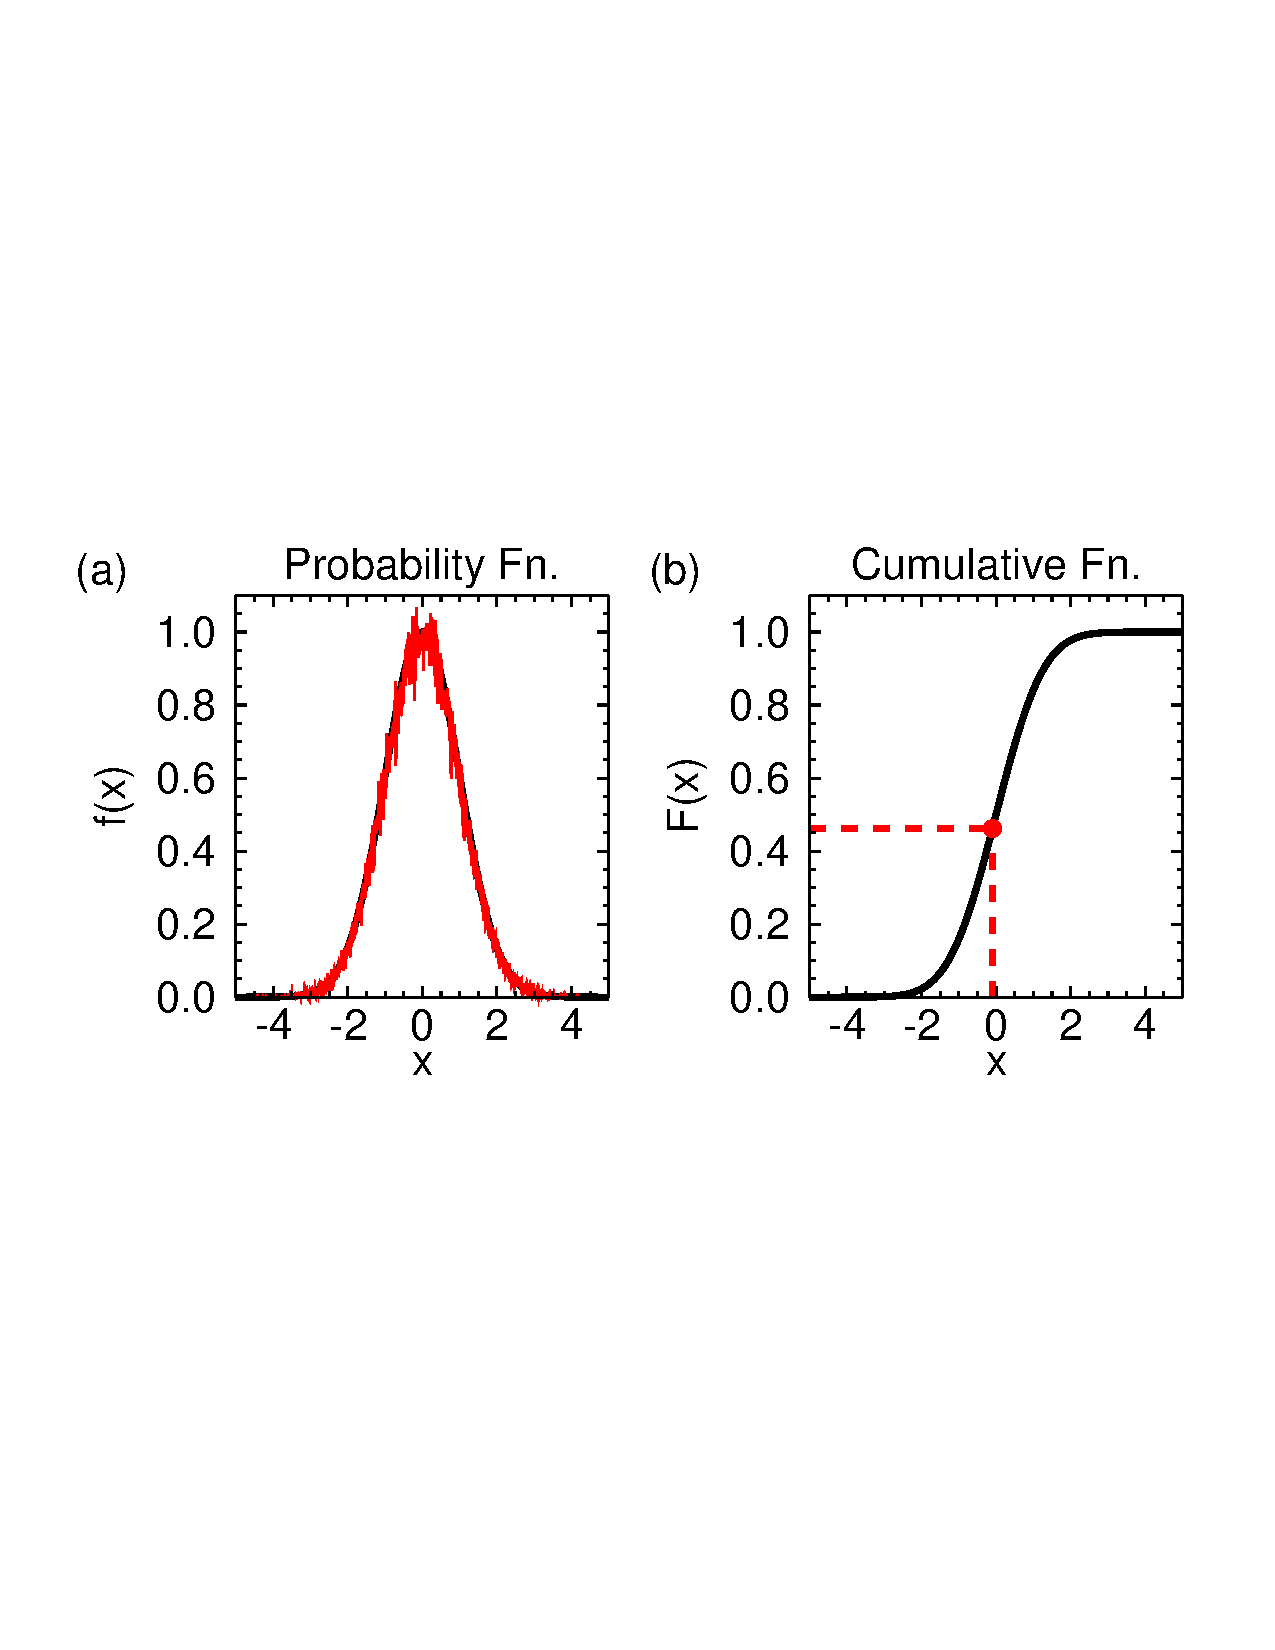
\includegraphics[width=6in]{probdist.pdf}
\caption{Transformation method to choose points from a probability distribution
function. (a) Specified probability distribution function (black) and histogram
of $10^5$ points chosen from this distribution (red). (b) Cumulative
distribution function (back). Red point shows a randomly drawn point from the
distribution. Random F(x)=0.46 implies x=-0.10.}
\label{fig:probdist}
\end{figure}

When using this method, the distribution needs to be well sampled, especially
around discontinuites, because the values on the cumulative distribution are
interpolated between the computed points.

Multivariate functions: P(x,y) = P(x)P(y)

Multivariate functions: P(x,y)

Spherical coordiates: P($\phi,\theta$)

\section{Appendix A: Directory Structure}

Directory structure as of 19 January 2010. Directories are listed in blue. IDL
program files are in black. Data files are in red. Data files ending in 
\textit{.dat} are ASCII format. Data files ending in \textit{.sav} are IDL save 
files. I've removed some files from this listing that don't do anything.

Notes: See Section~\ref{sec:AtomicData} for a description of atomic data files 
and lists of the available reactions and references.

\begin{enumerate}
\item {\color{blue}model\_pro\_2.0}
  \begin{enumerate}
  \item {\color{blue}AtomicData}
    \begin{enumerate}
      \item Lishawa\_crosssections.pro
      \item extract\_Berez\_data.pro
      \item extract\_Huebner\_data.pro
      \item find\_reactions\_2.0.pro
      \item make\_crosssec\_struct\_2.2.pro
      \item make\_ratecoef\_struct\_2.1.pro
      \item make\_reaction\_list\_2.1.pro
      \item rate\_func\_1.0.pro
      \item rate\_integral\_2.0.pro
      \item set\_default\_emission\_2.0.pro
      \item set\_default\_reactions\_2.0.pro
      \end{enumerate}
  \item {\color{blue}Data}
    \begin{enumerate}
    \item {\color{blue}CAPSplasma}
      \begin{enumerate}
      \item {\color{red}SaturnPlasma.2008-04-16.sav}
      \end{enumerate}
    \item {\color{blue}VoyagerTorus}
      \begin{enumerate}
      \item {\color{red}VoyagerTorus.sav}
      \item {\color{red}electrons.energetic.dat}
      \item {\color{red}electrons.thermal.dat}
      \item {\color{red}ions.energetic.dat}
      \item {\color{red}ions.thermal.dat}
      \item {\color{red}make\_plasma\_struct.pro}
      \end{enumerate}
    \item {\color{red}JupiterConstants.sav}
    \item {\color{red}MercDist.sav}
    \item {\color{red}MercuryConstants.sav}
    \item physical\_constants\_2.0.pro
    \item {\color{red}SaturnConstants.sav}
    \item SystemConstants\_2.0.pro
    \item {\color{red}SolarConstants.sav}
    \item atomicmass\_2.0.pro
    \end{enumerate}
  \item {\color{blue}Display}
    \begin{enumerate}
    \item density\_track\_2.0.pro
    \item line\_of\_sight\_2.5.pro
    \item model\_images\_2.6.pro
    \item model\_view.pro
    \item quick\_look.pro
    \item surface\_column\_density.pro
    \item zenith\_column\_2.0.pro
    \end{enumerate}
  \item {\color{blue}Docs}
    \begin{enumerate}
    \item manual.tex
    \item manual.pdf
    \end{enumerate}
  \item {\color{blue}Forces}
    \begin{enumerate}
    \item accel\_2.0.pro
    \item get\_gvalue\_2.1.pro
    \item gravity\_2.0.pro
    \item lorentz\_2.0.pro
    \item radiation\_pressure\_2.1.pro
    \end{enumerate}
  \item {\color{blue}Integrator}
    \begin{enumerate}
    \item driver\_2.5.pro
    \item impact\_check\_2.7.pro
    \item rk5\_2.0.pro
    \end{enumerate}
  \item {\color{blue}Lifetimes}
    \begin{enumerate}
    \item JupiterPlasma\_2.0.pro
    \item SaturnPlasma\_2.0.pro
    \item TorusState\_1.1.pro
    \item create\_lossinfo\_2.1.pro
    \item determine\_ratecoefs\_2.1.pro
    \item ionization\_rate\_3.0.pro
    \item lifetime\_setup\_2.3.pro
    \item load\_plasma\_2.0.pro
    \item make\_lifetime\_grid\_2.0.pro
    \item neutlt\_1.1.pro
    \item xyz\_to\_magcoord\_2.0.pro
    \end{enumerate}
  \item {\color{blue}Misc}
    \begin{enumerate}
    \item OTD.pro
    \item dipole\_field.pro
    \item dual\_dipoles.pro
    \item radial\_smooth.pro
    \item radial\_subtract.pro
    \item rotate\_packets.pro
    \item trace\_fieldline.pro
    \item trace\_normline.pro
    \end{enumerate}
  \item {\color{blue}SourceDistributions}
    \begin{enumerate}
    \item MonteCarloDistribution\_2.0.pro
    \item SO2exosphere\_distribution\_2.0.pro
    \item add\_perturbation\_2.2.pro
    \item angular\_distribution\_2.2.pro
    \item charge\_exchange\_perturbation\_2.0.pro
    \item exosphere\_distribution\_2.1.pro
    \item show\_veldist\_1.0.pro
    \item source\_distribution\_2.2.pro
    \item speed\_distribution\_2.4.pro
    \item speed\_dists\_2.0.pro
    \item surface\_distribution\_2.1.pro
    \item torus\_distribution\_2.0.pro
    \end{enumerate}
  \item {\color{blue}SystemViewer}  \\
    \textit{This directory is empty. I think I'm going to put my system viewer 
    widget in here when I get it cleaned up.}
  \item {\color{blue}Widget} \\
    \textit{Nothing in here works very well except the run\_widget.}
  \item combine\_iterations\_2.3.pro
  \item compress\_structs\_2.0.pro
  \item compile\_model\_2.0
  \item extract\_distribution\_2.0.pro
  \item inputs\_saverestore\_2.8.pro
  \item loc\_operations\_2.1.pro
  \item locmoon\_1.0.pro
  \item model\_common\_blocks\_2.0.pro
  \item modeldriver\_2.4.pro
  \item modstreamA\_2.3.pro
  \item modstreamB\_2.1.pro
  \item planet\_dist\_2.0.pro
  \end{enumerate}

\item {\color{blue}AtomicData}
  \begin{enumerate}
  \item{\color{blue}Emission}
    \begin{enumerate}
    \item {\color{blue}O}
    \item {\color{blue}O\_2}
    \item {\color{blue}S}
    \item {\color{blue}SO\_2}
    \item {\color{red}DefaultsList.dat}
    \item {\color{red}ReactionList.rate.dat}
    \item set\_up\_all\_reactions.pro
    \end{enumerate}
  \item{\color{blue}Loss}
    \begin{enumerate}
    \item {\color{blue}AlO}
    \item {\color{blue}C}
    \item {\color{blue}CH\_4}
    \item {\color{blue}CO}
    \item {\color{blue}CO\_2}
    \item {\color{blue}Ca}
    \item {\color{blue}CaO}
    \item {\color{blue}Cl}
    \item {\color{blue}FeO}
    \item {\color{blue}H}
    \item {\color{blue}H\_2}
    \item {\color{blue}H\_2O}
    \item {\color{blue}H\_2O+}
    \item {\color{blue}H\_3O+}
    \item {\color{blue}He}
    \item {\color{blue}K}
    \item {\color{blue}KO}
    \item {\color{blue}Mg}
    \item {\color{blue}MgO}
    \item {\color{blue}N}
    \item {\color{blue}NH\_3}
    \item {\color{blue}N\_2}
    \item {\color{blue}Na}
    \item {\color{blue}O}
    \item {\color{blue}OH}
    \item {\color{blue}O\_2}
    \item {\color{blue}S}
    \item {\color{blue}SO}
    \item {\color{blue}SO\_2}
    \item {\color{blue}SiO}
    \item {\color{blue}TiO}
    \item {\color{blue}multi-species}
    \item {\color{red}DefaultsList.dat}
    \item {\color{red}ReactionList.rate.dat}
    \item set\_up\_all\_reactions.pro
  \end{enumerate}
  \item{\color{blue}g-values}
    \begin{enumerate}
    \item {\color{red}CI.dat}
    \item {\color{red}CaI.dat}
    \item {\color{red}CaII.dat}
    \item {\color{red}HI.dat}
    \item {\color{red}HeI.dat}
    \item {\color{red}KI.dat}
    \item {\color{red}MgI.dat}
    \item {\color{red}MgII.dat}
    \item {\color{red}NaI.dat}
    \item {\color{red}OH.dat}
    \item {\color{red}OI.dat}
    \item {\color{red}SI.dat}
    \end{enumerate}
  \end{enumerate}
\end{enumerate}

\section{Appendix B: Inputfile Summary}

This appendix contains all the possibilities for each input. The lines can be 
copied and pasted into an input file as needed.

\subsection{Geometry}
\begin{itemize}
\item Mercury
  \begin{verbatim}
  geometry.planet = Mercury
  geometry.taa = 0.
  geometry.include = 1
  \end{verbatim}

\item Jupiter
  \begin{verbatim}
  geometry.planet = Jupiter
  geometry.startpoint = Io
  geometry.CML = 0.
  geometry.phi = 0.		;; Jupiter
  geometry.phi = 4.71239        ;; Io
  geometry.phi = 4.71239        ;; Europa
  geometry.phi = 4.71239        ;; Ganymede
  geometry.phi = 4.71239        ;; Callisto
  geometry.include = 1          ;; Jupiter
  geometry.include = 1          ;; Io 
  geometry.include = 0          ;; Europa
  geometry.include = 0          ;; Ganymede
  geometry.include = 0          ;; Callisto
  \end{verbatim}

\item Saturn
  \begin{verbatim}
  geometry.planet = Saturn
  geometry.startpoint = Enceladus
  geometry.phi = 0.             ;; Saturn
  geometry.phi = 4.71239        ;; Mimas
  geometry.phi = 4.71239        ;; Enceladus
  geometry.phi = 4.71239        ;; Tethys
  geometry.phi = 4.71239        ;; Dione
  geometry.phi = 4.71239        ;; Rhea
  geometry.phi = 4.71239        ;; Titan
  geometry.phi = 4.71239        ;; Hyperion
  geometry.phi = 4.71239        ;; Iapetus
  geometry.phi = 4.71239        ;; Phoebe
  geometry.include = 1          ;; Saturn
  geometry.include = 0          ;; Mimas
  geometry.include = 1          ;; Enceladus
  geometry.include = 0          ;; Tethys
  geometry.include = 0          ;; Dione
  geometry.include = 0          ;; Rhea
  geometry.include = 0          ;; Titan
  geometry.include = 0          ;; Hyperion
  geometry.include = 0          ;; Iapetus
  geometry.include = 0          ;; Phoebe
  \end{verbatim}
\end{itemize}

\subsection{Sticking\_Info}

\begin{itemize}
\item For everything to stick to the surface:
  \begin{verbatim}
  sticking_info.StickCoef = 1
  \end{verbatim}
\item For bouncing packets with thermal reemission:
  \begin{verbatim}
  sticking_info.StickCoef = 0
  sticking_info.emitfn = Maxwellian
  sticking_info.accom_factor = 1.
  sticking_info.Tsurf = 0
  \end{verbatim}
\item For bouncing packets to scatter elastically 
  \begin{verbatim}
  sticking_info.StickCoef = 0
  sticking_info.emitfn = elastic scattering
  \end{verbatim}
\end{itemize}

\subsection{Forces}

\begin{verbatim}
forces.gravity = 1
forces.radpres = 1
forces.lorentz = 0
\end{verbatim}

\subsection{SpatialDist}

\begin{itemize}
\item For packets spread across the surface (or uniform exobase) between a 
specified longitude and latitude range:
  \begin{verbatim}
  SpatialDist.type = surface
  SpatialDist.random_even = random
  SpatialDist.use_map = 0
  SpatialDist.exobase = 1.
  SpatialDist.longitude0 = 0.
  SpatialDist.longitude1 = 6.2831853
  SpatialDist.latitude0 = -1.5707963
  SpatialDist.latitude1 = 1.5707963
  \end{verbatim}
\item For packets spread across the surface (or uniform exobase) according to a
pre-specified probability distribution:
  \begin{verbatim}
  SpatialDist.type = surface
  SpatialDist.random_even = random
  SpatialDist.use_map = 1
  SpatialDist.mapfile = mapfile.sav
  SpatialDist.exobase = 1.
  \end{verbatim}
\item For packets distributed in a torus around the central planet
  \begin{verbatim}
  SpatialDist.type = torus
  SpatialDist.random_even = random
  SpatialDist.radius0 = 4.
  SpatialDist.radius1 = 1.
  SpatialDist.radius2 = 1.
  \end{verbatim}
\item For packets distributed in a spherically symmetric exosphere
  \begin{verbatim}
  SpatialDist.type = exosphere
  SpatialDist.exotype = powerlaw
  SpatialDist.b = -2
  SpatialDist.rmax = 10.
  SpatialDist.block_shadow = 0
  \end{verbatim}
\item For packets distributed according to Vincent Dol's SO$_2$ exosphere 
distribution:
  \begin{verbatim}
  SpatialDist.type = SO2 exosphere
  \end{verbatim}
\end{itemize}

\subsection{SpeedDist}

\begin{itemize}
\item Gaussian speed distribution
  \begin{verbatim}
  SpeedDist.type = Gaussian
  SpeedDist.vprob = 3.
  SpeedDist.sigma = 1.
  \end{verbatim}
\item Tri-gaussian speed distribution
  \begin{verbatim}
  SpeedDist.type = trigaussian
  SpeedDist.vxprob = 3.
  SpeedDist.vxsigma = 1.
  SpeedDist.vyprob = 2.
  SpeedDist.vysigma = 0.5
  SpeedDist.vzprob = 1.
  SpeedDist.vzsigma = 0.1
  \end{verbatim}
\item Sputtering speed distribution
  \begin{verbatim}
  SpeedDist.type = sputtering
  SpeedDist.U = 2.
  SpeedDist.alpha = 3
  SpeedDist.beta = 1.
  \end{verbatim}
\item Maxwellian at constant temperature
  \begin{verbatim}
  SpeedDist.type = maxwellian
  SpeedDist.temperature = 2000.
  \end{verbatim}
\item Thermal distribution at local surface temperature
  \begin{verbatim}
  SpeedDist.type = thermal
  \end{verbatim}
\item Equal probability for $v_{prob} \pm \Delta v$
  \begin{verbatim}
  SpeedDist.type = flat
  SpeedDist.vprob = 3
  SpeedDist.delv = 1.
  \end{verbatim}
\item Start packets in stable, circular orbits about the central planet
  \begin{verbatim}
  SpeedDist.type = circular orbits
  \end{verbatim}
\item Use Vincent Dol's SO$_2$ exosphere velocity distribution
  \begin{verbatim}
  SpeedDist.type = dolsfunction
  SpeedDist.dols0 = 1.
  SpeedDist.dols1 = 1.
  \end{verbatim}
\end{itemize}

\subsection{AngularDist}

\begin{itemize}
\item The speed distribution selected doesn't need an angular distribution to
be specified.
  \begin{verbatim}
  AngularDist.type = none
  \end{verbatim}
\item Send packets out radially from the central obeject
  \begin{verbatim}
  AngularDist.type = radial
  \end{verbatim}
\item Send packets out isotropically between specified altitude and azimuth
ranges
  \begin{verbatim}
  AngularDist.type = isotropic
  AngularDist.altitude0 = 0.
  AngularDist.altitude1 = 1.5707963
  AngularDist.azimuth0 = 0.
  AngularDist.azimuth1 = 6.2831853
  \end{verbatim}
\item Send packets out proportional to $\cos^n \theta$, where $\theta$ is the
altitude.
  \begin{verbatim}
  AngularDist.type = costheta
  AngularDist.n = 1.
  AngularDist.altitude0 = 0.
  AngularDist.altitude1 = 1.5707963
  AngularDist.azimuth0 = 0.
  AngularDist.azimuth1 = 6.2831853
  \end{verbatim}
\end{itemize}

\subsection{PerturbVel}

\begin{itemize}
\item Don't add a perturbation onto the initial velocity distribution.
  \begin{verbatim}
  PerturbVel.type = none
  \end{verbatim}
\item Add a Gaussian perturbation onto the initial velocity distribution.
  \begin{verbatim}
  PerturbVel.type = gaussian
  PerturbVel.vprob = 1.
  PerturbVel.sigma = 0.2
  \end{verbatim}
\item Add a tri-gaussian perturbation onto the initial velocity distribution
  \begin{verbatim}
  PerturbVel.type = trigaussian
  PerturbVel.vxprob = 1.
  PerturbVel.vxsigma = 0.2
  PerturbVel.vyprob = 1.
  PerturbVel.vysigma = 0.2
  PerturbVel.vzprob = 1.
  PerturbVel.vzsigma = 0.2
  \end{verbatim}
\item Use a charge exchage type perturbation
  \begin{verbatim}
  PerturbVel.type = charge exchange
  PerturbVel.flowvel = 10.
  \end{verbatim}
\end{itemize}

\subsection{plasma\_info}

\begin{itemize}
\item Mercury -- \textit{not used}
\item Jupiter
  \begin{verbatim}
  plasma_info.eps = 0.246
  plasma_info.thermal = 1
  plasma_info.energetic = 1
  \end{verbatim}
\item Saturn 
  \begin{verbatim}
  plasma_info.elecdenmod = 1
  plasma_info.electempmod = 1
  \end{verbatim}
\end{itemize}

\subsection{options}

\begin{verbatim}
options.packets = 30000
options.endtime = 36000
options.resolution = 1e-6
options.at_once = 0
options.atom = Na
options.lifetime = 0
options.fullsystem = 0
options.outeredge = 20.
options.motion = 1
options.trackloss = 0
options.datapath = $HOME/Data/AtomicData
options.modelpath = $HOME/Work/NeutralModel/modelpro_2.0
\end{verbatim}

\end{document}
